% mnras_template.tex 
%
% LaTeX template for creating an MNRAS paper
%
% v3.0 released 14 May 2015
% (version numbers match those of mnras.cls)
%
% Copyright (C) Royal Astronomical Society 2015
% Authors:
% Keith T. Smith (Royal Astronomical Society)

% Change log
%
% v3.2 July 2023
%	Updated guidance on use of amssymb package
% v3.0 May 2015
%    Renamed to match the new package name
%    Version number matches mnras.cls
%    A few minor tweaks to wording
% v1.0 September 2013
%    Beta testing only - never publicly released
%    First version: a simple (ish) template for creating an MNRAS paper

%%%%%%%%%%%%%%%%%%%%%%%%%%%%%%%%%%%%%%%%%%%%%%%%%%
% Basic setup. Most papers should leave these options alone.
\documentclass[fleqn,usenatbib,openbib]{mnras}

% MNRAS is set in Times font. If you don't have this installed (most LaTeX
% installations will be fine) or prefer the old Computer Modern fonts, comment
% out the following line
\usepackage{newtxtext}
\usepackage[varvw]{newtxmath}
% Depending on your LaTeX fonts installation, you might get better results with one of these:
%\usepackage{mathptmx}
%\usepackage{txfonts}

% Use vector fonts, so it zooms properly in on-screen viewing software
% Don't change these lines unless you know what you are doing
\usepackage[T1]{fontenc}

% Allow "Thomas van Noord" and "Simon de Laguarde" and alike to be sorted by "N" and "L" etc. in the bibliography.
% Write the name in the bibliography as "\VAN{Noord}{Van}{van} Noord, Thomas"
\DeclareRobustCommand{\VAN}[3]{#2}
\let\VANthebibliography\thebibliography
\def\thebibliography{\DeclareRobustCommand{\VAN}[3]{##3}\VANthebibliography}


%%%%% AUTHORS - PLACE YOUR OWN PACKAGES HERE %%%%%

\usepackage[spanish]{babel}
\usepackage{lipsum}
\usepackage{url}
\usepackage{pgfplots}
\usepackage{booktabs, colortbl, bigstrut, multirow}

% Only include extra packages if you really need them. Avoid using amssymb if newtxmath is enabled, as these packages can cause conflicts. newtxmatch covers the same math symbols while producing a consistent Times New Roman font. Common packages are:
\usepackage{graphicx}	% Including figure files
\usepackage{amsmath}	% Advanced maths commands
\usepackage{xfrac}

\usepackage{wrapfig}
\usepackage{cuted}
\usepackage[labelfont=bf,font=footnotesize]{caption}

%%%%%%%%%%%%%%%%%%%%%%%%%%%%%%%%%%%%%%%%%%%%%%%%%%

%%%%% AUTHORS - PLACE YOUR OWN COMMANDS HERE %%%%%

\usepackage[nameinlink,noabbrev]{cleveref}
\crefformat{figure}{\textsuperscript{#2#1#3}}
\crefformat{table}{\textsuperscript{#2#1#3}}

\addto\captionsspanish{\renewcommand{\refname}{REFERENCIAS}}

\makeatletter
\def\@abstract{\list{}{%
    \listparindent\realparindent
    \itemindent\z@
    \labelwidth\z@ \labelsep\z@
    \leftmargin\z@\rightmargin\z@%%was 11pc left
    \parsep 0pt plus 1pt}\item[]%
    \reset@font\normalsize{\bf PRESENTACIÓN}\\\reset@font\abslarge
} % SFB 0.1.01
\def\@keywords{\list{}{%
    \labelwidth\z@ \labelsep\z@
    \leftmargin\z@\rightmargin\z@  %was 11pc left was 11pc\right....
    \parsep 0pt plus 1pt}\item[]\reset@font\abslarge{\bf Palabras clave: }%
}
\makeatother

\renewcommand\theequation{\Alph{equation}}

% Redefine figure environment to allow manual placement specifier
\makeatletter
\renewenvironment{figure}[1][]{%
    \@float{figure}[#1]%
}{%
    \end@float
}
\makeatother

% Redefine table environment to allow manual placement specifier
\makeatletter
\renewenvironment{table}[1][]{%
    \@float{table}[#1]%
}{%
    \end@float
}
\makeatother

% Please keep new commands to a minimum, and use \newcommand not \def to avoid
% overwriting existing commands. Example:
%\newcommand{\pcm}{\,cm$^{-2}$}	% per cm-squared

%%%%%%%%%%%%%%%%%%%%%%%%%%%%%%%%%%%%%%%%%%%%%%%%%%

%%%%%%%%%%%%%%%%%%% TITLE PAGE %%%%%%%%%%%%%%%%%%%

% Title of the paper, and the short title which is used in the headers.
% Keep the title short and informative.
\title[Estudio de la Corriente y Resistencia Eléctrica]{Corriente y Resistencia Eléctrica}

% The list of authors, and the short list which is used in the headers.
% If you need two or more lines of authors, add an extra line using \newauthor
\author[Álvaro Jerónimo Sánchez]{
Álvaro Jerónimo Sánchez$^{1}$, DNI: 09847051S.\thanks{E-mail: alvaro.jeronimos@estudiante.uam.es}
Copartícipe: Hugo Pérez Hernández$^{1}$
\\
% List of institutions
$^{1}$Universidad Autónoma de Madrid, Ciudad universitaria de Cantoblanco, 28049,España \\
Facultad de Ciencias, Grado en Química, FÍSICA II
}

% These dates will be filled out by the publisher
\date{Prácticas 26/04/2024. Informe 09/04/2024. Fecha Límite 16/05/2024}

% Enter the current year, for the copyright statements etc.
\pubyear{2024}

% Don't change these lines
\begin{document}
\label{firstpage}
\pagerange{\pageref{firstpage}--\pageref{lastpage}}
\maketitle

%%%%%%%%%%%%%%%%%%%%%%%%%%%%%%%%%%%%%%%%%%%%%%%%%%

%%%%%%%%%%%%%%%%% BODY OF PAPER %%%%%%%%%%%%%%%%%%
\begin{abstract}

Mediante el estudio del comportamiento de diversos dispositivos ante distintos potenciales, se han observado cambios en la resistencia eléctrica de cada componente del circuito. En este trabajo se presentan resultados de las medidas tomadas, junto a la interpretación de las mismas, observando si los componentes cumplen o no la ley de Ohm.

\vspace{1cm}
\end{abstract}

%%%%%%%%%%%%%%%%%%%%%%%%%%%%%%%%%%%%%%%%%%%%%%%%%%
\section{Teoría}

La corriente eléctrica es un fenómeno que consiste en el flujo de partículas cargadas por un medio conductor. Cuando una partícula con carga se mueve en un campo eléctrico, éste ejerce una fuerza que efectúa trabajo sobre la partícula. A esta energía ejercida en forma de trabajo se le denomina energía potencial eléctrica, y el concepto que la representa expresada por unidad de carga se conoce como voltaje (o potencial eléctrico).

Al pasar por un material que no es totalmente conductor, presenta resistencia a la corriente, que dependerá de la resistividad del material, además del área transversal y longitud del segmento (\cite{Sears}). Los conceptos de voltaje, resistencia e intensidad los relaciona la ley de Ohm: $I=\frac{V}{R}$; no obstante, esta ley no es universal. En caso de observar una relación proporcional de estas magnitudes (al graficar $I$ sobre $V$, deberíamos observar una recta), el componente estudiado cumple la ley de Ohm.  En cambio, si se observase una gráfica de carácter exponencial, sería necesario aplicar logaritmos a distintas variables, buscando una relación lineal para deducir qué dependencia cumple (ver sección \ref{calculos}).

Los componentes que cumplen la ley de Ohm son denominados componentes \textit{óhmicos}, y la resistencia de éstos es independiente de la corriente que pasa a través de ellos y del voltaje (\cite{Ohm}). Éstos están siempre formados por sólidos como el cobre y el aluminio (la mayoría de los metales son óhmicos). Sin embargo, todos los conductores líquidos o gaseosos (además de algunos sólidos) son \textit{no óhmicos} (\cite{elec}). A pesar de esto, en corriente contínua su comportamiento se aproxima al de un material óhmico. Componentes como las lámparas incandescentes se esperan que no sean óhmicos, ya que su resistividad se ve afectada por la temperatura del material.

%%%%%%%%%%%%%%%%%%%%%%%%%%%%%%%%%%%%%%%%%%%%%%%%%%
\section{Montaje experimental}

\subsection{Material empleado}

Los dispositivos estudiados ($D$) han sido una resistencia óhmica (de valor desconocido), un diodo semiconductor y una lámpara incandescente. Para medir las caídas de potencial en los componentes se ha empleado un polímetro con un error de $\pm 5\, mV$. Tanto para la resistencia óhmica como para el diodo se ha introducido una resistencia $R_i$ de $470 \pm 1 \,\Omega$, y para la lámpara, se ha introducido una $R_i = 10\pm  0.3\,\Omega$. 

\begin{minipage}{0.5\columnwidth}
    \centering
    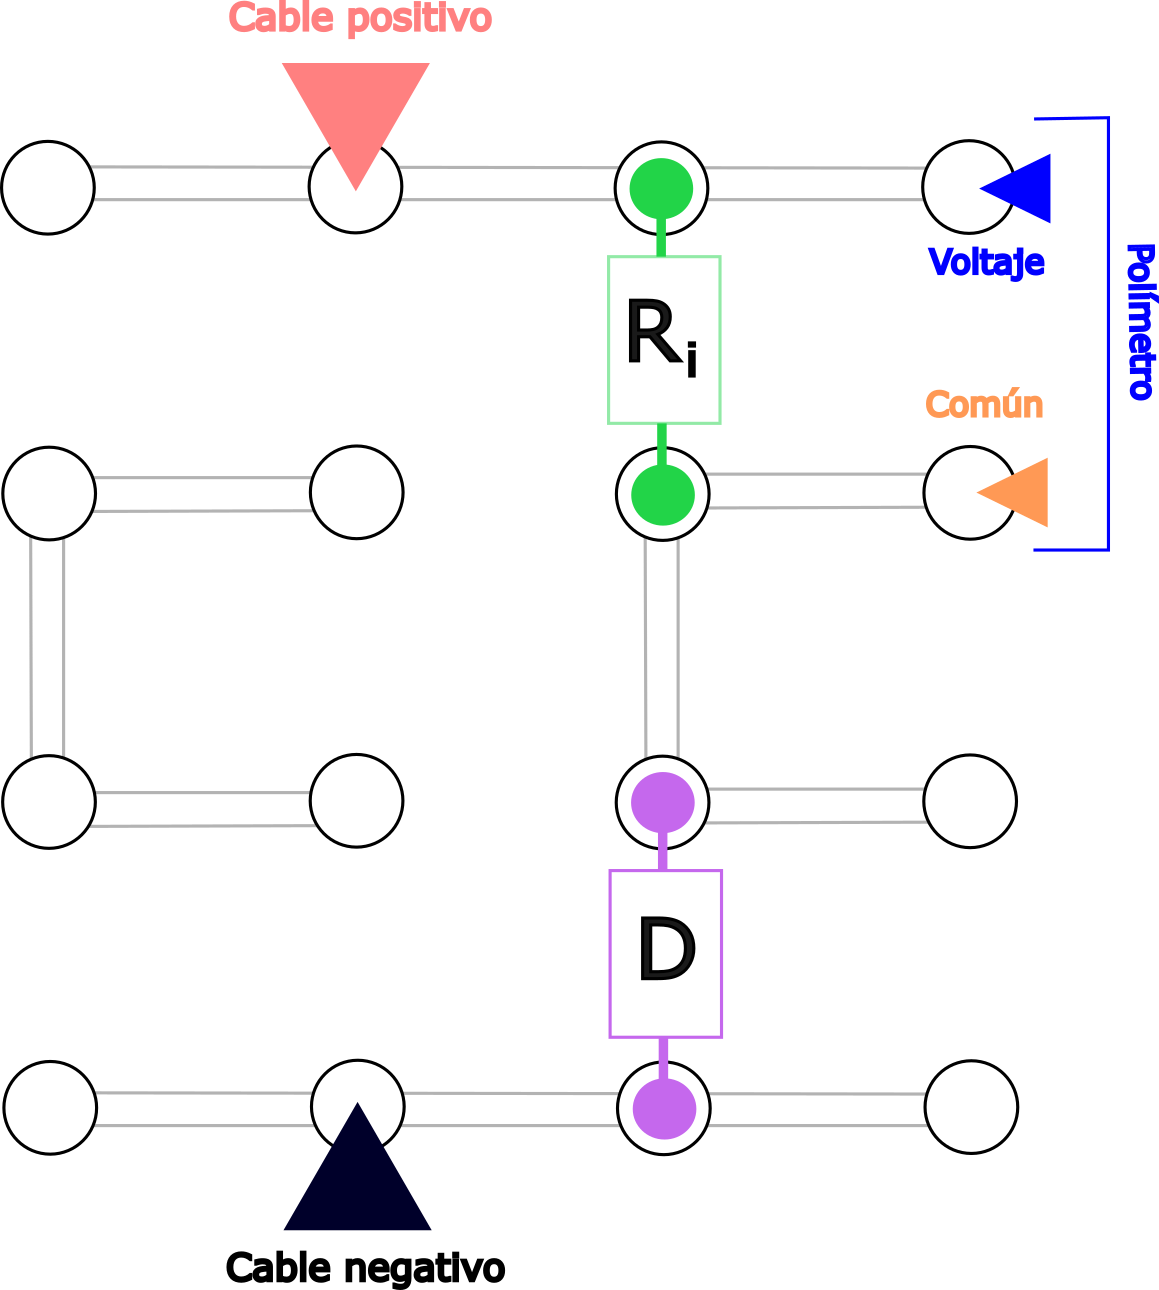
\includegraphics[width=0.8\columnwidth]{images/panel.png}
    \captionof{figure}{\\ Diagrama general del circuito}
    \label{fig:panel}
\end{minipage}
\begin{minipage}{0.4\columnwidth}
    Se ha montado el circuito en un panel de 4 x 4, colocando los cables de la fuente lo más cerca posible del resto de los componentes para minimizar errores. Inicialmente se han posicionado con el cable positivo en la parte superior del circuito (como se muestra en la figura \ref{fig:panel}). Para cada caso, se han tomado medidas de la caída de potencial en $R_i$ y en $D$.
\end{minipage}

\subsection{Medición}

A la hora de tomar las medidas, se ha repetido el mismo proceso en cada circuito. Primero se han colocado los componentes correspondientes en la placa de montaje y los cables de la fuente en la posición ilustrada en la figura \ref{fig:panel}. Esta posición ha permanecido constante en todos los casos hasta haber anotado todas las medidas, momento en el que se ha invertido la polaridad y se ha repetido la toma de datos. Para cada circuito, se ha empezado con el voltaje a 0, y se ha ido aumentando éste de uno en uno (en voltios) usando las perillas de la fuente: primero se ha manejado la perilla izquierda (que subía el voltaje en mayores incrementos), y a continuación se ha ajustado con más precisión empleando la derecha. Se han registrado medidas desde 0 a 15 $V$ para ambas polaridades.



%%%%%%%%%%%%%%%%%%%%%%%%%%%%%%%%%%%%%%%%%%%%%%%%%%
\section{Cálculos}
\label{calculos}

Una vez tomadas todas las medidas, se ha usado la ley de Ohm para hallar las intensidades en cada dispositivo:
\begin{gather}
    I=\frac{V}{R} \rightarrow I =\frac{V_{Ri}}{R_i} \label{eq:ohm}
\end{gather}

Se han graficado los valores de $I$ sobre $V_d$ de cada componente, y en el caso del resistor óhmico, que presentaba una relación lineal, se ha obtenido la resistencia que ésta suponía con la inversa de la pendiente de la recta (calculada con mínimos cuadrados por \textit{Excel}), ya que se ha graficado $I$ sobre $V_d$ y, por tanto:
\begin{gather}
    R=\frac{V_d}{I}=\frac{1}{m} \label{eq:m}
\end{gather}

En el resto de casos se ha tenido que aplicar logaritmos en las variables para encontrar dicha relación lineal (ver sección \ref{graphics}). 


\subsection{Errores}

\begin{center}
\fbox{
\begin{minipage}{0.65\linewidth}
\textsc{Errores de los inst: }

    $\bullet\Delta R_i$ ($470 \Omega$) = $\pm 1\, \Omega$\\
    $\bullet\Delta R_i$ ($10 \Omega$) = $\pm 0.3\, \Omega$ \\
    $\bullet\Delta$ Polím. = $\pm 0.001\, V$.
\end{minipage}}
\end{center}

Se ha calculado el error de la intensidad derivando la expresión despejada de la ley de Ohm (\ref{eq:ohm}), obteniendo:
\begin{gather}
    \Delta I = \left|\frac{\partial I}{\partial R_i}\right|\Delta R_i + \left|\frac{\partial I}{\partial V_{Ri}}\right|\Delta V_{Ri} \implies V_{Ri}\frac{1}{R_i^2}\Delta R_i + \frac{1}{R_i}\Delta V_{Ri}
\end{gather}

Para hallar el error de la resistencia (supuesta por el resistor óhmico) se ha empleado la función \textit{ESTIMACION.LINEAL} de \textit{Excel}, y se ha sustituido el error de la pendiente en la expresión que se halla derivando la ecuación \ref{eq:m}:
\begin{gather}
    \Delta R = \left|\frac{\partial R(m)}{\partial m}\right| \Delta m = \frac{1}{m^2}\Delta m \label{eq:mErr}
\end{gather}


\begin{strip}
\section{Resultados}

\subsection{Tabla de resultados}

    {\centering
    \includegraphics[width=0.9\textwidth]{images/data.png}
    \label{tab:data}
    \captionof{table}{Tabla de medidas registradas junto a los errores de la intensidad}}

\end{strip}

\begin{strip}
\subsection{Gráficas}
\label{graphics}

    {\centering
    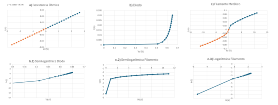
\includegraphics[width=0.9\textwidth]{images/graphics.png}
    \label{fig:graphics}
    \captionof{figure}{Gráficas $I$-$V_d$ de cada dispositivo (a-c) junto a las gráficas logarítmicas (b.2, c.2, c.3)}}

\end{strip}

En la gráfica de la \textbf{resistencia óhmica} se ha observado un carácter lineal, por lo que es el único dispositivo que \underline{\smash{cumple la ley de Ohm}}. Se ha realizado un ajuste de mínimos cuadrados con \textit{Excel}, resultando en la función $y=0.0099x-9\cdot 10^{-6}$. Como se ha mencionado en la sección \ref{calculos}, la resistencia supuesta por este componente corresponde con la inversa de la pendiente; por lo que el resultado \ref{eq:m} con su error \ref{eq:mErr} es:
\begin{gather*}
    R = \frac{1}{0.009892} \pm \frac{1}{0.009892^2}\cdot 3.66\cdot 10^{-5} = \boxed{101.01 \pm 0.37 \; \Omega} 
\end{gather*}

Se ha podido comparar este resultado con el valor obtenido observando las bandas de la resistencia. La secuencia de 4 bandas marrón-negro-marrón-dorado indica una resistencia de $1\;0\cdot 10 \pm 10 \implies 100\pm 10 \Omega$, lo que coincide con la cifra experimental con notable exactitud.
\\[12pt]
En el caso del \textbf{diodo} se ha observado que ha restringido la corriente a un sólo sentido, lo que se ve reflejado en la gráfica (\ref{fig:graphics} b). Es un comportamiento esperado, ya que es un semiconductor, y posee un área con exceso de electrones y otra con exceso de protones separadas por un área vacía. Esto provoca que sólo se pueda polarizar en un sentido y, por tanto, en el sentido contrario no dejará pasar la corriente (\cite{cien}). Al tener carácter exponencial, se ha aplicado un logaritmo neperiano a la intensidad, tras lo que se ha podido observar un carácter lineal (\ref{fig:graphics} b.2). Esto supone que la relación que cumple el diodo es:
\begin{gather*}
    R = \frac{V_d}{\ln(I)} \implies I = e^{\sfrac{V_d}{R}}
\end{gather*}

La gráfica del \textbf{filamento incandescente} (\ref{fig:graphics} c) tampoco describe una recta, por lo que se ha tenido que buscar dicha relación aplicando logaritmos. Al realizar la gráfica semilogarítmica (\ref{fig:graphics} c.2), se sigue viendo una trayectoria no lineal, y ha sido necesario hacer una logarítmica (\ref{graphics} c.3). En este caso, al haber aplicado logaritmos neperianos tanto en la intensidad como en el voltaje, la relación que cumple el filamento es:
\begin{gather*}
    R = \frac{\ln(V_d)}{\ln(I)} \implies I = e^{\sfrac{\ln(V_d)}{R}}
\end{gather*}

%%%%%%%%%%%%%%%%%%%%%%%%%%%%%%%%%%%%%%%%%%%%%%%%%%
\section{Conclusión}

Tras tomar medidas y observar los comportamientos de los distintos dispositivos, se ha concluido que sólo uno de ellos (la resistencia óhmica) cumple la ley de Ohm. Tanto el diodo como el filamento incandescente cumplían modulaciones de dicha ley, presentando logaritmos naturales en algunas de las variables. También se ha comprobado cómo el diodo limita el sentido de la corriente debido a ser un semiconductor, y como consecuencia se ha obtenido caída de potencial $0$ en el diodo al invertir el voltaje de la fuente. En el caso del filamento, no cumple la ley de Ohm porque la resistividad del material varía con la temperatura, cuyo incremento se podía observar claramente al aumentar el voltaje, ya que la lámpara brillaba más intensamente y el color de dicha luz fue cambiando de manera gradual de un rojo tenue hasta un amarillo anaranjado.

Como se ha discutido en la sección \ref{graphics}, también se ha conseguido hallar el valor de la resistencia óhmica con exactitud, ya que coincide con el que indican las bandas de colores.

%%%%%%%%%%%%%%%%%%%% REFERENCES %%%%%%%%%%%%%%%%%%

% The best way to enter references is to use BibTeX:

\vfill
\nocite{*}
\bibliographystyle{mnras}
\bibliography{bibliography}


% Alternatively you could enter them by hand, like this:
% This method is tedious and prone to error if you have lots of references
%\begin{thebibliography}{99}
%\bibitem[\protect\citeauthoryear{Author}{2012}]{Author2012}
%Author A.~N., 2013, Journal of Improbable Astronomy, 1, 1
%\bibitem[\protect\citeauthoryear{Others}{2013}]{Others2013}
%Others S., 2012, Journal of Interesting Stuff, 17, 198
%\end{thebibliography}

%%%%%%%%%%%%%%%%%%%%%%%%%%%%%%%%%%%%%%%%%%%%%%%%%%

%%%%%%%%%%%%%%%%% APPENDICES %%%%%%%%%%%%%%%%%%%%%
\clearpage
\appendix

\begin{strip}
\section*{Apéndice}
\label{appendix}
\centering

\captionof{figure}{Gráfica a mano en papel milimetrado $I$-$V_d$ de la resistencia óhmica}
\includegraphics[width=0.8\linewidth]{images/milim-resist.png}

\centering

\captionof{figure}{Gráfica semilogarítmica a mano en papel milimetrado $I$-$V_d$ del diodo}
\includegraphics[width=0.82\linewidth]{images/milim-diodo.png}

\end{strip}

%%%%%%%%%%%%%%%%%%%%%%%%%%%%%%%%%%%%%%%%%%%%%%%%%%


% Don't change these lines
\bsp	% typesetting comment
\label{lastpage}
\end{document}

% End of mnras_template.tex